\documentclass[12pt]{book}
\usepackage{hyperref}

\title{Physics of Complex Systems} \author{\url{https://github.com/Grufoony/Physics_Unibo}}
\date{}

\usepackage{amsmath}
\usepackage{amsfonts}
\usepackage{amssymb}
\usepackage{amsthm}
\usepackage{braket}
\usepackage[margin=3cm]{geometry}
\usepackage{pgfplots}
\pgfplotsset{compat=1.18}
\usepackage{fancyhdr}
\usepackage{physics}
\usepackage{systeme,mathtools}
\usepackage{graphicx}
\usepackage{float}
\usepackage{relsize}
\usepackage{calligra}
\usepackage{siunitx}
\usepackage{circuitikz}
\usepackage[miktex]{gnuplottex}
\usepackage{epstopdf}
\usepackage[english]{babel}
\usepackage{float}
\usepackage{tikz}


\newcommand{\vv}{\vec{v}}
\newcommand{\vw}{\vec{w}}
\newcommand{\vo}{\vec{0}}
\newcommand{\vx}{\vec{x}}
\newcommand{\R}{\Re}
\newcommand{\la}{\lambda}
\newcommand{\al}{\alpha}
\newcommand{\bd}{\textbf}
\newcommand{\lang}{\left\langle}
\newcommand{\rang}{\right\rangle}
\newcommand{\lbra}{\left\lbrace}
\newcommand{\rbra}{\right\rbrace}
\newcommand{\ih}{\hat{i}}
\newcommand{\jh}{\hat{j}}
\newcommand{\kh}{\hat{k}}
\newcommand{\vr}{\vec{r}}

\newtheorem{prop}{Proposition}
\newtheorem{definition}{Definition}

\makeatletter
\def\input@path{{./tex/}}
\makeatother

\begin{document}

\maketitle
\tableofcontents
\pagebreak

\chapter{Introduction to Complex Systems}
Complex systems are interdisciplinary: you have to communicate your results to experts from different science field.
You need to provide an easy answer to a complex problem, no matter how difficult it's to get this answer.
\section{Emergence}
One of the main ideas in complex systems is emergence. Emergence means that the structure of the particles is simple and they are not so important like interactions bettween them. \\
An example of this is the Central limit theorem, which comes from mathematics. \\ \\
If you have a random variable $x_k$, with average value $\lang x_k \rang = 0$ and finite variance $\sigma^2$, then the central limit theorem says that, if the variables are independent (and in physics this is usally a fair assumption) for every value of $k$, then the normalized sum 
$$
	z_n = \frac{1}{\sqrt{N}}\sum_{k=0}^N x_k
$$
then the distribution of this variable $z_n$ is known, and it is gaussian, for a big enough value of $N$.
$$
	\rho(z_n) \sim \exp\left(-\frac{z^2}{2\sigma^2}\right)
$$
Despite the fact that we, as humans, need a cause-effect relationship to describe a phenomenon, nature loves independent events, like DNA mutations.
The gaussian describes the fluctuations of a system at equilibrium, not the complexity. You cannot extract work from fluctuations at equilibrium, otherwise you violate thermodynamics (and that's no good). \\
The gaussian function is not a physical function, because it implies non zero probabilities to events which are impossible. For example, if we take a particle in a basin of attraction of a potential, the non zero probability given by the gaussian fluctuations allows the particle to jump out of the pit. But this violates the second law of thermodynamics. \\ \\
A way to defy the gaussian properties is to allow a system to have memory, so to remove the independence of the variable. 
\begin{center}
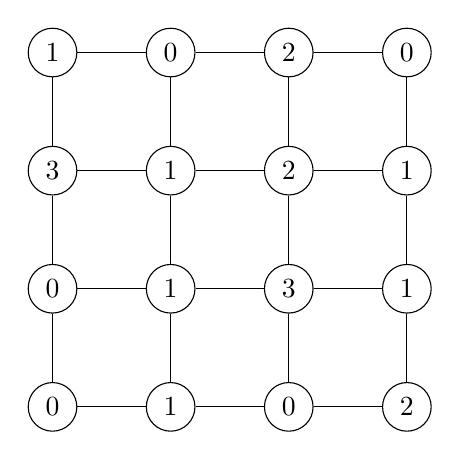
\begin{tikzpicture}[node distance={15mm}, main/.style = {draw,circle}]
\node[main] (1) {1};
\node[main] (2) [right of=1] {0};
\node[main] (3) [right of=2] {2};
\node[main] (4) [right of =3] {0};
\node[main] (5) [below of =1] {3};
\node[main] (6) [right of=5] {1};
\node[main] (7) [right of=6] {2};
\node[main] (8) [right of=7] {1};
\node[main] (9) [below of=5] {0};
\node[main] (10) [right of=9] {1};
\node[main] (11) [right of=10] {3};
\node[main] (12) [right of=11] {1};
\node[main] (13) [below of=9] {0};
\node[main] (14) [right of=13] {1};
\node[main] (15) [right of=14] {0};
\node[main] (16) [right of=15] {2};
\draw (1) -- (2);
\draw (1) -- (5);
\draw (2) -- (3);
\draw (3) -- (4);
\draw (5) -- (6);
\draw (6) -- (7);
\draw (7) -- (8);
\draw (5) -- (9);
\draw (9) -- (10);
\draw (10) -- (11);
\draw (11) -- (12);
\draw (9) -- (13);
\draw (13) -- (14);
\draw (14) -- (15);
\draw (15) -- (16);
\draw (2) -- (6);
\draw (3) -- (7);
\draw (4) -- (8);
\draw (6) -- (10);
\draw (7) -- (11);
\draw (8) -- (12);
\draw (10) -- (14);
\draw (11) -- (15);
\draw (12) -- (16);
\end{tikzpicture}
\end{center}
One example of this is the sand pile model. You have a lattice, and each point is connected to its four neighbors. At this point one particle is put in a randomly chosen point. Each node can have four possible states, $0,1,2,3$, that is four possible numbers of particles. If a node reaches 4 particles, the 4 particles are distributed to the 4 neightbouring nodes.
\begin{center}
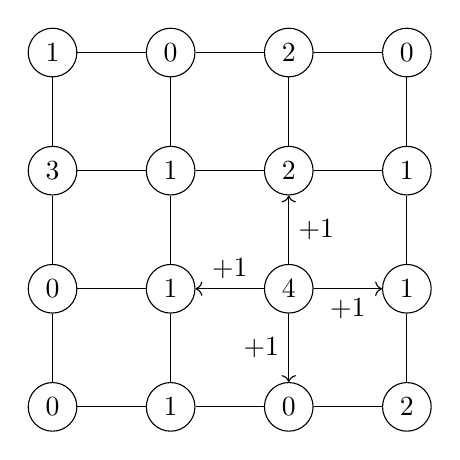
\begin{tikzpicture}[node distance={15mm}, main/.style = {draw,circle}]
\node[main] (1) {1};
\node[main] (2) [right of=1] {0};
\node[main] (3) [right of=2] {2};
\node[main] (4) [right of =3] {0};
\node[main] (5) [below of =1] {3};
\node[main] (6) [right of=5] {1};
\node[main] (7) [right of=6] {2};
\node[main] (8) [right of=7] {1};
\node[main] (9) [below of=5] {0};
\node[main] (10) [right of=9] {1};
\node[main] (11) [right of=10] {4};
\node[main] (12) [right of=11] {1};
\node[main] (13) [below of=9] {0};
\node[main] (14) [right of=13] {1};
\node[main] (15) [right of=14] {0};
\node[main] (16) [right of=15] {2};
\draw (1) -- (2);
\draw (1) -- (5);
\draw (2) -- (3);
\draw (3) -- (4);
\draw (5) -- (6);
\draw (6) -- (7);
\draw (7) -- (8);
\draw (5) -- (9);
\draw (9) -- (10);
\draw[->] (11) -- node[above]{+1} (10);
\draw[->] (11) -- node[below]{+1} (12);
\draw (9) -- (13);
\draw (13) -- (14);
\draw (14) -- (15);
\draw (15) -- (16);
\draw (2) -- (6);
\draw (3) -- (7);
\draw (4) -- (8);
\draw (6) -- (10);
\draw[->] (11) -- node[right]{+1} (7);
\draw (8) -- (12);
\draw (10) -- (14);
\draw[->] (11) -- node[left]{+1} (15);
\draw (12) -- (16);
\end{tikzpicture}
\end{center}
\begin{center}
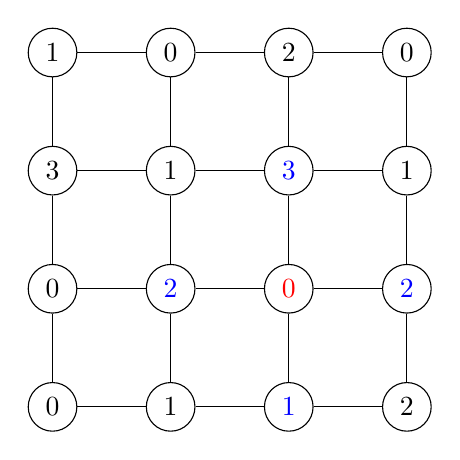
\begin{tikzpicture}[node distance={15mm}, main/.style = {draw,circle}]
\node[main] (1) {1};
\node[main] (2) [right of=1] {0};
\node[main] (3) [right of=2] {2};
\node[main] (4) [right of =3] {0};
\node[main] (5) [below of =1] {3};
\node[main] (6) [right of=5] {1};
\node[main] (7) [right of=6] {\textcolor{blue}{3}};
\node[main] (8) [right of=7] {1};
\node[main] (9) [below of=5] {0};
\node[main] (10) [right of=9] {\textcolor{blue}{2}};
\node[main] (11) [right of=10] {\textcolor{red}{0}};
\node[main] (12) [right of=11] {\textcolor{blue}{2}};
\node[main] (13) [below of=9] {0};
\node[main] (14) [right of=13] {1};
\node[main] (15) [right of=14] {\textcolor{blue}{1}};
\node[main] (16) [right of=15] {2};
\draw (1) -- (2);
\draw (1) -- (5);
\draw (2) -- (3);
\draw (3) -- (4);
\draw (5) -- (6);
\draw (6) -- (7);
\draw (7) -- (8);
\draw (5) -- (9);
\draw (9) -- (10);
\draw (11) -- (10);
\draw (11) -- (12);
\draw (9) -- (13);
\draw (13) -- (14);
\draw (14) -- (15);
\draw (15) -- (16);
\draw (2) -- (6);
\draw (3) -- (7);
\draw (4) -- (8);
\draw (6) -- (10);
\draw (11) -- (7);
\draw (8) -- (12);
\draw (10) -- (14);
\draw (11) --  (15);
\draw (12) -- (16);
\end{tikzpicture}
\end{center}
For the nodes in the border, what happens is that 2 of the particles are redistributed and the other 2 are released in the enviroment, so they are lost. \\ \\
So this system has memory, and this means that the states of all the nodes are not independent. This memory turns the gaussian distribution into a power law
$$
	p(n) \propto n^{-\alpha}
$$
with $\alpha > 1$. \\
The decay of the power low is much slower than that of the gaussian, which means that the probability to have events in the extremes is significantly higher with the power low distribution.
Memory is related to power laws, but vice versa is not guaranteed.
We can also have power laws in physics, for example in the Ising model.
In physics, power laws typically represent a phase transition for a dynamic system in a non-equilibrium state. \\
In the sand pile model, we notice a self-organized criticality: the system naturally goes into a critical state and does a phase transition. \\
Another example of a natural power law is the Kleiber law which relates the metabolic rate (amount of energy you need to survive) to the mass.
\begin{equation}
	E(m) \propto m^{\frac{4}{3}}
\end{equation}
We can also observe that heartbeat rate decreases with mass and lifetime increases.
\section{Network's energy}
Let's take a region of space containing a number $N$ of nodes. This system can represent, for example, the hydraulic network of a city. 
For a node we define its ``energy'' flow $\varphi$ (in the case of the hydraulic network, what is flowing between the nodes is water). How much ``energy'' do we need to insert in the system? \\
If we have to distribute something to all the nodes, the most basic way to do it is to connect one on one all the nodes, as to form a long chain. \\
\begin{center}
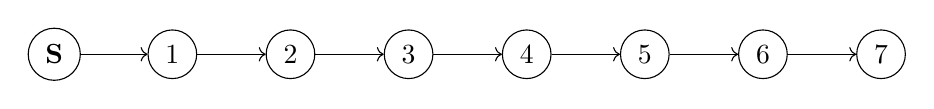
\begin{tikzpicture}[node distance={15mm}, main/.style = {draw,circle}]
\node[main] (1) {1};
\node[main] (0) [left of=1] {\textbf{S}};
\node[main] (2) [right of=1] {2};
\node[main] (3) [right of=2] {3};
\node[main] (4) [right of =3] {4};
\node[main] (5) [right of =4] {5};
\node[main] (6) [right of=5] {6};
\node[main] (7) [right of=6] {7};
\draw[->] (0) -- (1);
\draw[->] (1) -- (2);
\draw[->] (2) -- (3);
\draw[->] (3) -- (4);
\draw[->] (4) -- (5);
\draw[->] (5) -- (6);
\draw[->] (6) -- (7);
\end{tikzpicture}
\end{center}
If the flow out of the source $S$ is $\phi$, the flow after the first node is $\phi - \varphi$, and so on, and we expect that the flow arriving to the final node will be $\varphi$. \\
So the total energy is 
$$
	E_T \approx l\sum_{k=0}^{N-1} (\phi - k\varphi) = l\varphi\sum_{k=0}^{N-1} k`
$$
$$
	E_T \propto l\varphi N^2
$$
So the totaly energy that is required to provide for all the nodes, with this configuration, is proportional to the square of the total number of nodes. So with this configuration we have a network that is very easy to implement, but the network is very inefficient. \\ \\ 
Another possible connection of the nodes is the following one:
\begin{center}
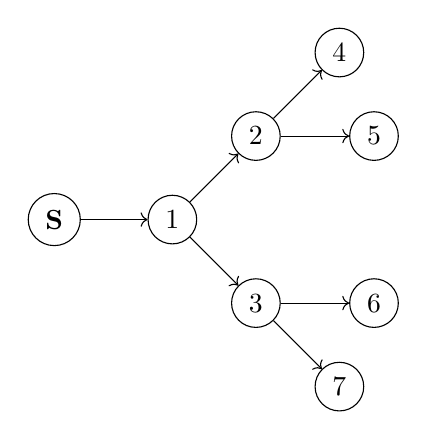
\begin{tikzpicture}[node distance={15mm}, main/.style = {draw,circle}]
\node[main] (1) {1};
\node[main] (0) [left of=1] {\textbf{S}};
\node[main] (2) [above right of=1] {2};
\node[main] (3) [below right of=1] {3};
\node[main] (4) [above right of =2] {4};
\node[main] (5) [right of =2] {5};
\node[main] (6) [right of=3] {6};
\node[main] (7) [below right of=3] {7};
\draw[->] (0) -- (1);
\draw[->] (1) -- (2);
\draw[->]  (1) -- (3);
\draw[->]  (2) -- (4);
\draw[->]  (2) -- (5);
\draw[->]  (3) -- (6);
\draw[->]  (3) -- (7);
\end{tikzpicture}
\end{center}
So each node is linked to two mode nodes. This is what is called a tree structure. \\
The main problem with such a structure is that the path between the nodes is always the same, but it is impossible to design a city in such a way. \\
The number of nodes is $N = 2^{m+1}$, where $m$ is the number of levels. \\
The relation for the flow in each level is
$$
	2\phi_k + \varphi = \phi_{k-1}
$$
where we assume again that the flow in the final level is $\varphi$. \\
$\phi_k$ then is
$$
	\phi_k = (2^{m+1-k}-1)\varphi
$$
Then:
$$
	E_T = d\varphi\sum_{k=1}^m 2^k(2^{m+1-k}-1) \approx d\varphi m 2^{m+1}	
$$
$$
	E_T = d\varphi N \log_2N
$$
This configuration is much more efficient than the previous alternative, although it is impossible to put to practice. \\ \\ 
So we need to find a solution that is in the middle of these two. \\ \\
Another possible structure consists of connecting all the nodes to the source, making a star network: also this model is of course impossible to put in practice. \\
However, in this case the total energy required is proportional to $NL$, where $L$ is the scale length of the system. 
$$
	E_T \propto NL
$$
The proportionality to $L$ is due to the fact that the average length of the links is proportional to the size of the space. \\
Since 
$$
	N = \left(\frac{L}{l} \right)^D
$$
where $D$ is the system dimension (e.g. 1D, 2D...).
We have that
$$
	E_T \propto N\overline{L} \approx N^{1+1/D} = V^{\frac{D+1}{D}}
$$
We notice that:
\begin{itemize}
	\item for a 2D system, like a city, $E \propto V^{\frac{3}{2}}$
	\item for a 3D system, like biological systems, $E \propto V^{\frac{4}{3}}$
\end{itemize}
In any case the exponent is greater than one so, soon or later, the system will collapse.
The problem is also logistic, because in a real transportation line there is also waste, that has to be disposed of. \\ \\
If we consider our system to be an animal's body, this would mean that in order to survive the amount of blood in its body must grow with the size by an amount of $4/3$. This would mean that very big animals can't survive, but they do, and the solution is in Kleiber's law. \\
As animals get bigger, their demand of energy goes down, so their metabolism slows down.  


Once we have a model (which hopefully is a good one), the model is deterministic, so if we know the initial conditions os the system, we know exactly what state the system will have at any future time. \\
The problem with this is that we don't know the initial conditions with absolute certainty. So at this point the question, that will be answered later, is: \\
How much error in the initial conditions is acceptable before that the previsions of our model start to diverge from the real evolution in an unacceptable way?
\section{Broken Stick Model}
Let's consider the portion $[0,1]$ of the axis, which represents a segment (a stick) of length 1. Suppose that we extract randomically a point $x_1$ on that segment, and we cut it in correspondence of that point, thus obtaining the portion $[0,x_1]$ of the axis. \\
By repeating this process many times, we obtain a system with memory, because of course the length of the segment at a certain iteration depends on all the previous iterations. \\
This is called the broken stick model. \\
For this system one expects to have a power law distribution, because if we rescale the variable $x$, the distribution must not change.
$$
	p(x) \sim \frac{1}{x^a}
$$
$$
	y = \la x \ \ \longrightarrow \ \ p(y) = \frac{1}{(\la x)^a} \sim \frac{1}{x^a}
$$
Since we have:
$$
	\lang x_k \rang = \frac{\lang x_{k-1} \rang}{2}
$$
$$
	\rho_N(2x) = \frac{1}{2}\rho_{N-1}(x)
$$
Which means that, as $N$ goes to infinity we get
$$
	\rho(2x) = \frac{1}{2}\rho(x)
$$
$$
	\rho(x) = \frac{1}{x}
$$
Let's now try to implement the system without memory. So we have $N$ independent variables $x_k$ uniformly distributed, and for each variable we define its distance from the previous one, $\Delta x$. \\
The probability to find $\Delta x$ is the probability of not finding $x$ in any segment, so
$$
	p(\Delta x) \approx \left( 1 - \frac{\Delta x}{L} \right)
$$
We then take a new variable $y = N\Delta x$ and we obtain the probability distribution
$$
	p = \exp(-y/L)
$$
as $N$ goes to infinity, which of course is an exponential law. \\ \\
Suppose that the whole stick is a state, and we want to distribute the population inside of it. If we divide the stick uniformly in portions and diivde the populations in this group, we obtain an exponential law, as we have just seen. \\
Another way, which contains memory, consists of creating a city and letting it grow, and only then introducing a second one, and repeating the process until all the space is occupied. 

\section{Rankings}
A ranking is an ordered subset of measures of the same quantity, between which exists an order relation. Rankings allow us to obtain complex informations with the use of very little data, since the information is contained in the order of the values. \\ 
An example of the use of rankings can be found in web pages, where the search engine shows to the user the results of the search, and the results are ordered depending on their relevance, so to allow them to find the desired information as quickly as possible. \\
In this example, the quantity is the relevance of a result to the search. \\ \\
Another example is the population of cities. The graph below shows the population of the 300 bigges cities in Europe. The graph is in log-log scale, and since it shows a straight line, it means that the distribution is a power law distribution. \\
\begin{center}
	\includegraphics[scale=0.65]{cities_ranking.jpg}
\end{center}
This can be explained considering the fact that, storically, the population used to migrate towards the biggest cities of the country, because there were more job opportunities. Thus one can say that big cities have a preferential attatchment. \\ \\ 
Let $x$ be a random variable and $\{x_1,x_2, . . . , x_N\}$ a sample of experimental observations of the variable, ordered in such a way that $x_1 \geq x_2 \geq . \ . \ . \ \geq x_N$. \\ 
Then, the ranking distribution is created by assigning to the position $j$ in the order the corresponding value in the sampe, which is given by the map $x_j = f(j)$. Also, usually the elements are normalized like $y_j = x_j/x_1$. \\ 
By definition, $j/N$ is the frequency of the event $\{x \ | \ x \geq x_j \}$, that is, the probability that the variable $x$ has a value larger that $x_j$ for larger values of $j$. \\ \\
The cumulative distribution is defined as $F(x) = P\{u \ | \ u \leq x_j\}$, that is, the probability that the value $u$ is smaller that $x$. Of course, this probability is equal to the integral of the distribution in the range $[-\infty,x]$. \\
The relation between the frequency $j/N$ and the cumulative distribution is given by:
$$
	F(x_j) = 1 - \frac{j}{N} = 1 - \frac{J(x_j)}{N}
$$
where $J(x_j)$ is the inverse of the ranking, so it's the function that returns the position of a certain value of $x$ in the sample's order. \\
Since the cumulative distribution is the integral of the probability distribution, the latter can be obtained by differentiating the first:
$$
	p(x) = \frac{dF}{dx} \ \ \longrightarrow \ \ p(x) = -\frac{1}{N} \frac{dJ}{dx}
$$

\section{Laplace problem}
Let's suppose that we are tossing a coin, and the probability of gettin head is $p$ and the probability of getting tails is $1-p$. The event $E$ is $x_{n+1}$ outcome, and $H_n$ is $\{x_1,x_2,...\}$, so the first is the future and the second is the past. \\
Now we ask ourselves what is the probability that the next result of the toss is going to be heads:
$$
	p(x_{n+1}=H | H_n) 
$$
The most intuitive way to calculate this probability would be to use the frequentistic definition, so to count how many times we have gotten heads over the entire number of tries (we are considering the number of tries to be very big of course)
$$
	p = \frac{n_H}{N}
$$
Unfortunately, this is not the right way to do it. \\ \\
The probability of getting a given sequence of heads and tails is
$$
	p(\{x_k\}) = p^J(1-p)^{n-J}
$$
where $J$ is the number of times that we get heads. \\
Now if we integrate we get
$$
	\int_0^1 p^J(1-p)^{n-J}dp = \frac{J!(n-J)!}{(n+1)!}
$$
so
$$
	p(x_{n+1}=H|\{\}) = \frac{(n+1)!}{J!(n-J)!}p^J(1-p)^{n-J}
$$
which is a binomial distribution. \\
Now we calculate the average value of the probability
$$
\int_0^1 p\frac{(n+1)!}{J!(n-J)!}p^J(1-p)^{n-J}dp = \frac{J+1}{n+2}
$$
and we see that it isn't $J/n$, as one would have expected. 

\chapter{Basic models}
\section{Linear models}
The most simple model possible is the linear model
$$
	\dot{x} = Ax
$$
Albeit this model is easy, there are a few complications that have to be taken into account:
\begin{itemize}
	\item When the number of dimensions increases it becomes complicated. 
	\item If we consider the determinant
$$
	det(\la I - A) = 0
$$
we obtain a polinomial equation, that can be very hard to solve. 
	\item To further complicate things, $A$ might not be known, but we could have an ensemble of matrices. 
	\item The point $x=0$ is always a critical point, so we can always linearize the system around this point, but if $A$ has critical points then we get those as well. 
\end{itemize}
By solving the determinant equation, we get the eigenvalues $\la$, whose study can tell a lot about the behaviour of the solutions. \\
If $Re \la \leq 0$, this means that the exponential term of the solution shrinks, so it converges. \\ \\
Robustness means that if we perturb the system, the solutions don't change too much. A model must be robust, otherwise it can fit any kind of data simply by slightly changing the parameters. \\ \\
The formal way to write the solution of such a linear system is
$$
	x(t) = x_0\exp(At)
$$
For coefficients $\la^*$ such that $Re\la^* > 0$, we have that
$$
	|\delta x| \approx |e^{\la^* t}||\delta x_0|
$$
This is very tipical, and from this rises the chaos theory. In this case, even a small error in the initial condition will increase the error in the model exponentially fast. \\ \\
We get another interesting model by adding some noise to the linear model
$$
	\dot{x} = Ax + \xi(t)
$$
We consider a special solution of the form
$$
	x = e^{At}y
$$		
and we substitute in the equation
$$
	\dot{x} = A\exp(At)y + \xi(t) = A\exp(At)y + \exp(At)\dot{y}
$$	
$$
	\dot(y) = \exp(-At)\xi(t)
$$
So the complete solution of the problem is
\begin{equation}
	x(t) = \exp(At)x_0 + \int_0^t \exp(A(t-s))\xi(s)ds
\end{equation}
If the system is stable (negative real part of lambda) and we use a periodic forcing, the solution is still a periodic function with different period. \\ \\
Now we want to consider the case of a perturbed matrix:
$$
	\dot{x} = (A+\varepsilon B)x
$$
with $\varepsilon \ll 1$. \\
The solution is
$$
	x(t) = \exp((A+\varepsilon B) t)x_0
$$
and to understand the system's sensitivity we calculate the derivative for small perturbations
$$
	\frac{d}{d\varepsilon}\exp((A+\varepsilon B)t)
$$
but the problem is that usually the two matrices are not commutative. \\
If we take the special solution $x = \exp(At)x_0$ and we substitute we get
$$
	\dot{y} = \varepsilon\exp(-At)B\exp(At)y
$$
and, if $A$ and $B$ do not commute, this equation is very difficult to solve. \\
An approximate solution is
$$
	y(t) = y_0 + \varepsilon\int_0^t \exp(-As)B\exp(As)y_0ds + O(\varepsilon^2)
$$
and the solution for x is
\begin{equation}
	x(t) = \exp(At)x_0 + \varepsilon\int_0^t \exp(A(t-s))B\exp(As)x_0ds + O(\varepsilon^2)
\end{equation}
Now, the sensitivity of the system is
$$
	\frac{dx}{d\varepsilon} = \int_0^t \exp(A(t-s))B\exp(As)x_0ds 
$$
In the particular case where the matrix is diagonal, the sensitivity becomes
$$
	\frac{dx}{d\varepsilon} = \int_0^t \exp(\la_i(t-s))B_{ij}\exp(\la_js)x_0ds 
$$

\section{The neuron model}
In this model we have two variables, $x$ and $w$, and two differential equations to describe their dynamics
$$
	\dot{x} = x - \frac{x^3}{3} - w + I(t)
$$
$$
	\dot{w} = \frac{1}{\mu}(x+a-bw)
$$
This system is of course not linear, because we have a cubic term in the dynamics of $x$. \\
We require $\mu$ to be big, so that $w$ is the slow variable, whereas $x$ is the fast variable. \\
The fact that the two variables have different growth speeds is quite important, because it allows us to study them separately, and this reduces the complexity of the system. \\
The difference in the speed of the variables makes the system stiff, which means that it's very hard to integrate numberically. \\ \\
The key to studying this system is in the nullcline. We find the two nullclines by putting the two derivatives equal to zero, so one is a straight line and the other one is a cubic. \\
The two nullclines intersect, and the point where they intersect is the equilibrium point of the system. Furthermore, the cubic nullcline has two critical points. Since $x$ is the fast variable, the point follows the cubic nullcline in its dynamics. Once it reaches one of the two critical points, during its motion, it jumps to the other branch of the nullcline. So in the end one gets a periodic motion. \\ \\
Suppose now that $I(t)$ is of the form
$$
	I(t) = I_0 + \Delta I \delta(t)
$$	
so we give an impulse to the point. \\
What happens now is that, if $\Delta I$ is small, the point oscillates briefly around the critical point and falls back into it, but if the the impulse is big, the point excapes and makes a very big oscillation. \\
In this system we have an Hopf bifurcation. \\
\subsection{Hopf Bifurcation}
Sometimes the orbits of a dynamical system converge not in a single point but in limit circle near the stable point.
This is called \emph{Hopf Bifurcation}.
That type of phenomena is recurrent in nature: one example may be the Ising's model in which the system passes from a one stable point state to a two stable points state with a phase transition.
In that specific case we observe a bifurcation of the system's free energy.\\
We have to see the Hopf bifurcation as a new dynamical state that has a periodic orbit as a solution.
However, it's important to observe that a Hopf bifurcation is not an equilibrium state for the system.\\
For example, consider a circular network of identical neurons characterized by a function $\dot{x}_k$.
The dynamic is described by a simple law
$$
    \dot{x}_k=F(x_k)+\epsilon x_{k-1}
$$
in which the function F() is taken from the Fitzhug-Nagumo model and the other term represents the system dynamic.\\
If $x_P$ is an equilibrium point for all neurons then we can verify that exists an $\epsilon=\epsilon_C$ that produces a non-trivial solution.
In particular, with that value of $\epsilon$ we can create a stationary periodic state with a periodic signal (moving wave): that's a self-solution for the system.
Obviously, this example do not conserve the total energy of the system.

\chapter{Dynamical Systems}
% chaotic dynamics
A dynamical system is given by a \emph{phase space} $M \subseteq \mathbb{R}^d$ endowed with a collection of maps $\phi^t:M\rightarrow M$, where $t \in \mathbb{G} = \lbra \mathbb{R}, \mathbb{C}, \mathbb{Z}, \mathbb{N} \rbra$, with the so-called ``group property'':
$$
	\phi^{t+s} = \phi^t o \phi^s
$$
The maps $\phi^t$ are usually called \emph{flows}. \\ 
This formalization works for systems whose equations don't depend explicitly on time. \\
A typical example of a dynamical system is that of the solutions of a differential equation. So if we have a Cauchy problem
$$
	\begin{cases}
		\dot{x} = f(x) \\
		x\left(0\right) = x_0
	\end{cases}
$$
where the flow is the function that takes the initial condition and returns the correct solution for the differential equation.
So if this ODE has a global solution $x(t)$ that satisfies the initial condition, then 
$$
	\phi^t(x_0) = x(t)
$$
We must also assume the uniqueness of the solution, that is, for one initial condition we only have one solution. \\
Non-autonomous ODEs, where the equation field depends on time
$$
	\dot{x} = f(x,t)
$$
can be converted into autonomous ODEs in higher dimensions, going back to the previous simpler case. \\
We consider $\overline{M} = M \times \mathbb{R}$ with $y = (x,t) \in \overline{M}$, and we define
$$
	F(x,t) = (f(x,t),1)
$$
with $f : M \times \mathbb{R} \rightarrow \mathbb{R}^d$ and $F : M \times R = \overline{M} \rightarrow \mathbb{R}^{d+1}$. At this point we can write the new differential equation:
$$
	\dot{y} = F(y)
$$
with initial condition $y(0) = (x_0,0)$. For this to be useful, we must show that knowing the solution to this new equation implies knowing the solution for the original one. \\
Say $y(t) = (x(s),t(s))$ is a solution for the new equation
$$
	\left(\begin{matrix}
		\dot{x}(s) \\ 
		\dot{t}(s)
	\end{matrix}\right) = 
	F
	\left(\begin{matrix}
		x(s) \\ 
		t(s)
	\end{matrix}\right) =
	\left(\begin{matrix}
		f(x(s),t(s)) \\ 
		1
	\end{matrix}\right) = 
$$
$$
	\dot{x} = f(x,s) \ \ \ \ \ \dot{t} = 1
$$
with initial conditions $x(0) = x_0$ and $t(0) = 0$. For what concerns t, it's the identity function, so $t(s) = s$, which means that I can invert $t$ and $s$, so going back to the first equation we have
$$
	\dot{x} = f(x,t)
$$
which was our original equation. This means that a solution for the non-autonomous equation is also a solution for the new autonomous one. \\
So, if we have a theory that treats non-autonomous systems, that theory must also be able to treat autonomous systems. \\ \\
If the $t$ variable is a natural number, we call it $n$
$$
	\phi^n = T^n
$$
\section{Malthus model}
Let's take the expression
$$
	x_{n+1} = \alpha x_n
$$
where $x_n$ represents the population in year $n$. For $\alpha > 1$, we have population growth and for $\alpha < 1$ the population decreases. \\
If at time $t=0$ the population is $x_0$, at a given time we have
$$
	x_n = T_n(x_0) = \alpha^n x_0
$$
\section{Velhurst model}
This model takes into account the fact that the higher the population is, the more resources are needed, so there should be a limit that can't be surpassed, because the environment wouldn't be able to sustain it
$$
	x_{n+1} = \alpha x_n(A-x_n)
$$
Now we change variable, defining $y = x/A$, and we get
$$
	\frac{x_{n+1}}{A} = A\alpha \frac{x_n}{A}\left(1 - \frac{x_n}{A}\right)
$$
$$
	y_{n+1} = r y_n(1-y_n)
$$
which is the logistic map:
\begin{equation}
	T(x) = rx(1-x)
\end{equation}
We take $0 < x < 1$ and $1 < r < 4$. The graph is a parabola upside down, with the maximum at $\left(\frac{x}{2},\frac{r}{4}\right)$.
It may happen that $T\left(x\right)^n=x$: in this case the orbit $O\left(x\right)=\lbra\Phi^t\left(x\right)\rbra_{x \in \mathbb{G}}$ is called \emph{periodic orbit}.
We also observe that getting closer to an orbit is not the same as getting closer to a limit.
\section{Expanding map}
Now let's see an example of a chaotic map.
First of all, we define a map $T$ as \emph{expanding} if $\left\lvert T'\left(x\right)\right\rvert > 1$ $\forall x \in \mathcal{M}$.
As well, we also give this definition for a generic point:
\begin{definition}
    We define a periodic point of the map $x_0 \in \mathcal{M}$ as:
    \begin{itemize}
        \item \emph{attractive} if $\left\lvert T'\left(x_0\right)\right\rvert > 1$
        \item \emph{repelling} if $\left\lvert T'\left(x_0\right)\right\rvert < 1$
        \item \emph{neutral} if $\left\lvert T'\left(x_0\right)\right\rvert = 0$
    \end{itemize}
\end{definition}
For example, let's take the map $T : \left[0,1\right] \to \left[0,1\right]$ such as $T\left(x\right)=2x \ mod \ 1$.
This map as two fixed points (intersection with the bisectrice): $p_0 = \left(0,0\right)$ and $p_1 = \left(1,1\right)$.
We notice immediately that those points are both \emph{repelling} points.
Another thing we can see with this particular map is that if we start on a slightly different point from the previous one, for example $x \to x + \epsilon$, the difference between the two orbit grows exponentially fast:
$$
    T^n\left(x\right)=2^n\left(x-k\left(x\right)\right)-k\left(T\left(x\right)\right)
$$
where
$$
    k\left(x\right)=
    \begin{cases}
        0 \quad 0\leq x \leq \frac{1}{2} \\
        1 \quad \frac{1}{2} < x \leq 1
    \end{cases}
$$
and in conclusion we have that
$$
    T\left(x + \epsilon\right)=2^n\left(x + \epsilon\right) \ mod \ 1
$$
so the difference grows $\propto 2^n\epsilon$.
One last comment to make is that it's true that the two orbit exponentially diverges one from the other but the phase space is limited: from this point of view their distance in phase space will oscillate through time.


\begin{prop}
    If $T : \left[0,1\right] \to \left[0,1\right]$ is an expanding map such as $\left\lvert T'\left(x\right)\right\rvert > 1$ $\forall x \in \left[0,1\right]$ then any point p of $T^j$ ($j \in \mathbb{Z}$) is repelling.
\end{prop}
\begin{proof}
	If we take the derivative of $T^j$ we get
	$$
		(T^j)'(x) = T'(T^{j-1}(x))\times T'(T^{j-2}(x))\times...\times T'(x) = \prod_{k=0}^{j-1}T'\left(T^k\left(x\right)\right)
   $$
  	and if now we calculate the module of this derivative we get 
   $$
       \left\lvert\left(T^j\right)'\left(x\right)\right\rvert = \prod_{k=0}^{j-1}\left\lvert T'\left(T^k\left(x\right)\right)\right\rvert \gg 1
   $$
	where, since the map is expanding, each term of the product is larger then one.
\end{proof}
\begin{prop}
    If two points p and q are part of the same periodic orbit then they are both of the same type.
\end{prop}
\begin{proof}
    Let's consider an orbit of period $j$ with $q=T^k\left(p\right)$, $0 < k \leq j-1$.
    $$
        \left(T^j\right)'\left(p\right) = T'\left(p_0\right)\ldots T'\left(p_{j-1}\right)
    $$
    $$
        \left(T^j\right)'\left(q\right) = \left(T^j\right)'\left(p_k\right) T'\left(p_k\right)\ldots T'\left(p_{k-1}\right) \ldots T'\left(p_{k+j-1}\right)
    $$
    Real numbers always commute, so it's obvious that
    $$
        \left(T^j\right)'\left(q\right) = \left(T^j\right)'\left(p\right)
    $$
\end{proof}
We have just shown that the property of a point (local) is also a property of an orbit (global).

\section{Classification of chaotic systems}
% classification of chaotic systems
Let $\pi^1$ be a one-dimensional thorus (a circle). We define the transformations 
$$
	R_\alpha : \pi^1 \rightarrow \pi^1, \ R_\alpha(x) = (x + \alpha) \ mod \ 1
$$
which are called rotations by an ``angle" $\alpha$. \\
Now, if $\alpha = p/q$, with $\gcd(p,q)=1$, then:
\begin{itemize}
	\item all orbits are periodic with fundamental period $q$. 
	\item if $\alpha$ is not rational, then all orbits are dense. 
\end{itemize}
\begin{proof}
	\begin{itemize}
		\item We consider that $R^n_\alpha(x)=x$ is equivalent to $(x + n\alpha) \ mod \ 1 = x$, so 
		$$ 
			\left(x + n\frac{p}{q}\right) \ mod \ 1 = x
		$$
		which means that, 
		$$
			n\frac{p}{q} = k \ \longrightarrow	\ n = \frac{kq}{p}
		$$
		and for $n$ to be an integer, p needs to be simplified, but it can't be simplified with $q$, so it simplifies with $k$, which is then equal to $k = mp$. So in the end we get
		$$
			n = mq
		$$
		\item In order to prove that all orbits are dense, we prove that they are $\varepsilon-dense$ for all $\varepsilon$. \\
		Since $\alpha$ is not rational, the orbit must be infinite, because it is not periodic. Then, we can say that there is at least one accumulation point in the orbit. \\
		Now, call $j = n - m$, then we can say that $\{R^{k_j}_\alpha\}_k$ is $\varepsilon-dense$ in $\pi^1$, which means that the orbit is dense.
	\end{itemize}
\end{proof}
\subsection{Topological transitivity}
\begin{definition}
	A dynamical system $(M,\phi^t)$ is called topologically transitive (or just transitive) if exists $x\in M$ such that the future orbit
	$$
		O^t(x) = \{\phi^t(x)\}
	$$
	is dense.
\end{definition}
So a transitive system is a system that has at least one dense orbit. Going in that direction, if all the orbits are dense we say that the system is minimal.
\begin{definition}
	A system is called minimal if all forward orbits $O^t(x)$ are dense. 
\end{definition}
Another very important definition is that of an invariant subset:
\begin{definition}
	A subset $A \subseteq M$ is called invariant if $\phi^{-t}(A) = A$ for every $t$. \\
	Note that if $\phi^t$ is invertible, this statement is equivalent to saying that $\phi^t(A) = A$ for every $t$.
\end{definition}
Finding invariant subsets is important because we know that if we have an initial condition in that region, the orbit is going to stay in there. Of course, this doesn't give us the trajectory, but it helps us by restricting the phase space. \\ \\
A function $f:M\rightarrow R$ (observable) is called invariant if $f\circ\phi^t = f$ for every $t \geq 0$. This is what is called in mechanics a prime integral of motion. \\
Suppose $f = 1_a$, where $1_a(x) = 1$ if $x\in A$ and $1_a(x) = 0$ if $x \notin A$. Then we have that
$$
	1_a \circ \phi^t = 1_a
$$
but also 
$$
	1_a \circ \phi^t = 1_{\phi^{-t}(A)}
$$
So combining the two we get that 
$$
	\phi^{-t}(A) = A
$$
\begin{prop}
	If a dynamical system is topologically transitive, there exists no continuous invariant observables other than constant functions.
\end{prop}
%proof
\begin{proof}
	Say that $O^t(x_0)$ is dense. Now, taking any $y \in M$, we can say that exists a sequence $x_j = \phi^{t_j}(x_0)$ such that $x_j \longrightarrow y$. \\
	Now, suppose that a function $f$ is continuous, then
	$$
		f(x_j) \longrightarrow f(y)
	$$
	and suppose that $f$ is invariant, so that
	$$
		f(x_j) = f(\phi^{t_j}(x_0)) = f(x_0) = C
	$$
	Since we have taken $f$ to be continuous, $f(x_j)$ must converge to $f(y)$, but since it is constant and equal to $C$, it can only converge to $C$, which means that
	$$
		f(y) = C
	$$
	which is a constant function.
\end{proof}
\subsection{Rotation on a d-thorus}
Now we try to generalize rotations of the circle to translations of a d-thorus. \\
We define the translation on a d-thorus $T_\gamma$ as:
$$
	T_\gamma : \pi^d \rightarrow \pi^d, \ T_\gamma (x) = (x_1 + \gamma_1, x_2 + \gamma_2, ...) \ mod \ 1 = (x + \gamma) \ mod \ 1
$$
\begin{definition}
	A collection of real numbers $\{\la_1,\la_2,...\}$	is said to be \textit{rationally independent} if none of them can be written as a combination of the others with rational coefficients.
\end{definition}
Now that we have defined the concept of rational dependence, we can use it to introduce a characteristic of the translations on d-thori in the case where the vector components are rationally independent:
\begin{prop}
	Given a translation on a d-thorus $T_\gamma$, it is minimal if and only if $\{1,\gamma_1,\gamma_2,...\}$ are rationally independent. 
\end{prop}
% obs
In this case, topological transitivity (so the fact that the system hase one dense orbit) is equivalent to minimality (so all the system's orbits are dense). \\ 
This is due to the fact that translations commute. In fact, if we define a translation of the initial point $x_0$
$$
	T_{x-x_0}(x_0) = x
$$
then we see that translating the orbit of $T_\gamma$ starting from $x_0$ gives an orbit which is identical to the orbit starting from $x$: 
$$
	O^t(x_0) = O(x)
$$
$$
	T_{x-x_0} O^t(x_0) = T_{x-x_0}(T^k_\gamma(x_0)) = T^k(T_{x-x_0}(x_0)) = O(x)
$$
which means that the translated orbit is dense if and only if the initial one is dense, so translating a dense set we get another dense set. \\ \\
So we only need to show topological transitivity, instead of minimality. Let's show that topological transitivity implies rational independence: By contradiction, suppose that $1,\gamma_1,\gamma_2,...$ are not rationally independent, which means that exists a set $k_1,k_2,...$, where $k_i$ are not all zero, such that
$$
	\sum_i k_i\gamma_i = 0
$$
We then define the function $f(x) = e^{2\pi i \lang k,x\rang}$, which is continuous and non constant, because not all $k_i$ are zero (so you have at least one $x_i$ in the exponent). Now we just need to show that $f$ is invariant. To do this we calculate $f(T_\gamma(x))$:
$$
	f(T_\gamma(x)) = \exp(2\pi i \lang k, x + \gamma \rang) = \exp(2\pi i \sum_i k_ix_i)\exp(2\pi i \sum_i k_i \gamma_i) 
$$
$$
	= \exp(2\pi i \sum_i k_ix_i) = f(x)
$$
and this holds for every $x$ in the thorus. \\ \\
% poincarre sections
Let's take a system on a ring, and the dynamics represents rotations on this ring. We can imagine this as a cave tube filled with fluid (marmellade). In this case, the motion of the fluid will be laminar. \\
In discrete time, we take a surface with codimension 1, which is intersects the trajectory in a point $x$, and we want to find after how many iterations the trajectory intersects the surface again, so in other words, how long it's going to take for the trajectory to intersect the surface again. \\
A Poincarre section of a continuous dynamical system is a codimension 1 submanifold such that all trajectories cross it transversally (more or less). \\
In this case, the so called Poincarre map, also known as first return map, is defined as follows:
$$
	T_{M_0}: M_0 \rightarrow M_0, \ T_M(x) = \phi^{t_{M_0}(x)}(x) = \min \{t > 0 | \phi^t(x)\in M_0\}
$$
where $t_{M_0}$ is the return time to $M_0$.

\subsection{The Kronecker flow}
Continuous time dynamical system, the Kronecker flow.
$$
	\phi^t : \pi^d \rightarrow \pi^d
$$
given by the solutions of the ODE
$$
	\dot{x} = \omega
$$
In this case it's very easy to find the flux, which is simply
$$
	\phi^t(x) =  (x + \omega t) \ mod \ 1
$$
In general terms, suppose that $\omega = (\omega_1,\omega_2,...,\omega_d)$ with $\omega_d > 0$. Then the bottom side of the thorus $M_0$ is
$$
	M_0 = \{(x_1,x_2,...,x_{d-1},0)\in \pi_d \} = \pi_{d-1}
$$
and we know that all trajectories must cross this subspace. \\
The first return map is 
$$
	T_{M0}:M_0 \rightarrow M_0, \ T_{M0}(x) = \phi^{t_{M0}(x)}(x) = x + \frac{\omega}{\omega_d} \ mod \ 1
$$
This is the same as
$$
	T_\gamma : \pi^{d-1} \rightarrow \pi^{d-1}
$$
with $\gamma=(\omega_1/\omega_d,\omega_2/\omega_d,...)$. \\
Now we ask ourselves, when are the orbits of $T_\gamma$ dense? The answer is that they are when $\gamma_1,\gamma_2,...,\gamma_{d-1},1$ are rationally independent. But this condition is met if and only if $\omega_1,...,\omega_d$ are rationally independent. \\
This means that the trajectories of $\phi^t$ are dense if and only if $\omega_1,...,\omega_d$ are rationally independent.

\subsection{Important map}
$$
	T_2(x) = T(x) = 2x \ mod \ 1
$$
We can think of this map as either a map that goes from $[0,1]$ to itself, or as a map on a thorus. Alternatively it can be written as
$$
	T(x) = 2x, \ 0 \leq x \leq \frac{1}{2}
$$
$$
	T(x) = 2x-1, \ \frac{1}{2} \leq x \leq 1
$$
If we consider it as a map on a thorus, it is quite easy to see that this map is continuous. \\
As we have seen, this map is chaotic. To understand, if we consider two points $x_1$ and $x_2$, positioned at a distance $\varepsilon$, their distance after one iteration becomes $4\varepsilon$. \\

We understand that after a number of iterations these two points diverge pretty quickly, no matter how small we take $\varepsilon$ to be. \\
We write $x$ as $x = 0.d_1d_2d_3$, where $d_i$ are the digits. It can be written as
$$
	x = \sum_i^{\infty} 2^{-i}d_i
$$
We define the map $T(x)$ as 
$$
	T(x) = T(0.d_1d_2d_3) = 0.d_2d_3
$$
\begin{definition}
	A topological dynamical system (a system for which we care about topological properties) is said to be topologically mixing if $\forall U,V$ non-empty open sets, $\exists N = N(U,V) \in N$ such that 
	$$
		\phi^t(U) \cap V \neq \emptyset
	$$
	for all $t$.
\end{definition}
\begin{prop}
	$(M,\phi^t)$ is topologically transitive if and only if $\forall U,V$ non-empty open sets $\exists N = N(U,V)$ so that $\phi^N(U)\cap V \neq \emptyset$.
\end{prop}
A corollary of this proposotion is that topological mixing implies topologically transitive. \\ \\
We want to show that this map is topologically mixing. We know that a set, which is the arc connecting two points, expands in length after each iteration, and after a certain point it will fill the whole circle, and at that point it will keep being the whole circle, and in that case it's obvious that the intersection is not null. So we just need to prove that after a certain number of iteration the expanded set will fill the whole circle. \\
The function after $n$ iterations is
$$
	T^n(x) = 2^n(x) \ mod \ 1
$$
For any $n$
$$
	T^n(\left[\frac{k}{2^n},\frac{k+1}{2^n}\right]) = [0,1] = \pi^1
$$
Since $U$ is open, exists an $n$ with $0 < k < 2^n - 1$ such that $\left[\frac{k}{2^n},\frac{k+1}{2^n}\right]) \subset U$ \\ \\
% non ho capito
The number of periodic points of period $n$ of this map are $2^n - 1$. 

\subsection{Arnold's cat map}
$$
	T : \pi^2 \rightarrow \pi^2, \ T(x) = T(x_1,x_2) = A (x_1,x_2) \ mod \ 1
$$
where $A$ is the matrix
$$
	A = \begin{pmatrix}
		2 & 1 \\
		1 & 1
	\end{pmatrix}
$$
If we look how the points $(1,0)$ and $(0,1)$ transform, we see that they go to $2,1$ and $(1,1)$. \\
This map preserves the Lebesgue measure $\mu$
$$
	\mu(T^{-1}B) = \mu(B)
$$
If the system is bijective, this is the same as saying
$$
	\mu(TB) = \mu(B)
$$
so we can go forward in time. We know that the measure is preserved because $\det A = 1$. \\
We study the eingenvalues and eigenvectors of this matrix. These are $\la_1 = \la = \frac{3+\sqrt{5}}{2}$ and $\la_2 = \la^{-1} = \frac{3-\sqrt{5}}{2}$, with corresponding eigenvectors $(1,\frac{\sqrt{5}-1}{2})$ and $(1,-\frac{\sqrt{5}+1}{2})$. \\
The two eigenvectors represent the directions of maximum expansion and of maximum contraction. \\
If we take a point on the expanding eigenvector, its orbit diverges from the origin, whereas for a point on the contracting eigenvector the orbit is attracted to the origin. If we take a point which is a linear combination of the two directions, after each iteration the point gets closer and closer to the expanding eigenvector, because the component along the contracting eigenvector gets smaller after each iteration, and eventually it will disappear.
\begin{prop}
	The cat map $T_A$ is topologically mixing.	
\end{prop}
This map is an example of an "hyperbolic dynamical system". Let's call 
$$
	W^u(x) = \{y=(y_1,y_2)\in \pi^2| y_2-x_2 = \frac{\sqrt{5}-1}{2}(y_1-x_1) \ mod \ 1\}
$$
where $x$ are constants, an unstable manifold. Then we can define the stable manifold as
$$
	W^s(x) = \{y=(y_1,y_2)\in \pi^2| y_2-x_2 = -\frac{\sqrt{5}+1}{2}(y_1-x_1) \ mod \ 1\}
$$
Why do we expect systems like this to have a lot of periodic orbits?
Because of the stretching and folding mechanism. To see this, let's consider an hyperbolic rectangle, which is made up of pieces of stable manifolds in some points and unstable manifolds in other points. Now, we apply our dynamics to it, so the unstable manifolds will stretch and the stable ones will contract. \\
So if we have the rectangle $R$ and the transformed rectangle $R'=T(R)$, $R'$ will cross $R$ ad some point, with the condition that we can't have unstable manifolds crossing other unstable manifolds. Once we have found the intersection of the original rectangle and the transformed rectangle, we have found a fixed point of the transormation, hence we have found a periodic point, which implies the existence of a periodic orbit.








\chapter{Ergodic theory}
Ergodic theory is the study of dynamical systems from the point of view of measure theory, hence of probability. \\
One first measure comes from analytical mechanics. We consider a measure space $M$, and in this space we have an energetic hypersurface. Then we define the Liouville measure as
$$
	d\mu = \frac{d\sigma}{|\nabla H|}
$$
where $d\sigma$ is the measure of an infinitesimal portion of the hypersurface and $\nabla H$ is the gradient of the hamiltonian of the system. \\
We can derive the expression for the Liouville measure by considering the hypersurface with a bit of thickness in the direction of the gradient, forming in this way a volume $A$, and of course the system's dynamics is going to conserve the Lebesgue measure of $A$
$$
	Leb(A^t) = Leb(\phi^t(A)) = Leb(A)
$$
If we then move in the direction of the gradient by a quantity $h$, we increase the energy by a quantity
$$
	\Delta H = |\nabla H|h
$$
Then the conservation of the Lebesgue measure implies that
$$
	\sigma(B^t)h^t = \sigma(B)h
$$
so we are not only on the same energy surface, we are in the same energy shell. We can write this as
$$
	\frac{\sigma(B^t)\Delta H}{|\nabla H_f|} = \frac{\sigma(B)\Delta H}{|\nabla H_i|}
$$
and we can simplify the delta, so
$$
	\frac{\sigma(B^t)}{|\nabla H_f|} = \frac{\sigma(B)}{|\nabla H_i|}
$$
and we have thus obtained the expression for the Liouville measure. \\ \\ 
In ergodic theory we consider the space, along with the measure and the systems flux, $(M,\mu,\phi^t)$, or in discrete time $(M,\mu,T)$. \\
The first thing that we could ask ourselves is the probability that $\phi^t \in A$. So now we don't consider a single trajectory but all the possible trajectories, and want to find the probability that they are contained in a certain portion of space. This probability is equal to 
$$
	P(\phi^t \in A) = \mu(\phi^{-t}(A)) = \mu(\{x\in M \ | \ \phi^t(x) \in A\})
$$
A this point we can define the concept of a measure preserved by the dynamics
\begin{definition}
	A measure is preserved by the dynamics if 
	$$
		\mu(\phi^{-t}(A)) = \mu(A)
	$$
	where $A$ must be measurable, so it must belong the the $\sigma-$algebra of the space.
\end{definition}
From now on we restrict to measures that preserve the dynamics, which are also called invariant measures. \\ \\
An example of a measure preserving dynamical system is the doubling map. To see this, if we take the counter image of a set $A$, this is equal to the union of two sets $A_1$ and $A_2$, which are measurable. In this case it is important to consider the counter image of the set, because the image wouldn't preserve the set
$$
	\mu(TA) \neq \mu(A)
$$
When the two are equal, we have forward preservation. \\
An observable is any function of the phase space, $f:M \rightarrow R$, that represents any quantity of the system that can be observed and measured, thus giving us information about the system. An observable could the the temperature in a room, the moment of a particle or anything really.
\begin{definition}
	An observable $f:M \rightarrow R$ is said to be dynamics invariant (in ergodic theory) if
	$$
		f \circ \phi^t(x) = f(x)
	$$
\end{definition}
We notice that this is equivalent to the definition that we had before, but in the study of dynamical systems we asked for the relation to hold for every value of $x$, but we can't do this in ergodic theory, because not all the points in the space are seen by the measure. In ergodic theory we say that a relation holds if it holds almost everywhere, that is, if it doesn't hold only on subsets of the space that have zero measure. \\ \\
We also define the concept of an invariant set.
\begin{definition}
	A set $A$ is invariant if
	$$
		\phi^t(A) = A \ mod \ \mu
	$$
	We can also write it as
	$$
		\mu(\phi^{-t}A \Delta A) = 0
	$$
	where 
	$$
		A \Delta B = (A\cup B) \ (A \cap B)
	$$
\end{definition}
We then define push-forward measures:
\begin{definition}
	We define a push-forward measure as
	$$
		\phi^t * \mu(A) = \mu(\phi^{-t}(A))
	$$
\end{definition}
The measure contains the counter image because we are considering the points at an initial time and this allows us to require that they will be in the set at forward times. We can say, in probability terms, that the probability of being in $A$ at time $t$ is the same as the probability of being in $A$ at previous times. \\ \\	
Now we can note that a measure $\mu$ is preserved by the dynamics if an only if
$$
	\phi^t * \mu = \mu
$$
Now, if $\phi^t * \mu \rightarrow \nu$, then $\nu$ is called an equilibrium measure.
\section{Birkhoff's ergodic theorem}
Given an observable $f:M\rightarrow M$ we define the Birkhoff (time) average as
$$
	f^*(x) \ \lim_{t\rightarrow \infty} \frac{1}{T}\int_0^T f\circ \phi^t(x)dt
$$
The Birkhoff theorem states that:
\begin{prop}
	Given a measure preserving dynamical system $(M,\mu,T)$ with $\mu(M)=1$, if $f\in L^1(M,\mu)$, then 
	\begin{itemize}
		\item the limit $f^*$ exists almost everywhere
		\item 
			$$
				\int_M f^* d\mu = \int_M f d\mu
			$$
	\end{itemize}
\end{prop}
\begin{definition}
	A measure preserving dynamical system is ergodic if and only if for every $f\in L^1$ exists $c$ such that $f^*(x) = c$ for almost all values of $x$. 
\end{definition}
\begin{prop}
	The following statements are equivalent:
	\begin{itemize}
		\item $\forall f\in L^1$, $f^* = const$	
		\item $\forall f\in L^1$, $f^* = \int f d\mu$
		\item if $f \in L^1$ is invariant, then it is constant
		\item if $A \subseteq M$, which we take to be measurable, is invariant, the measure is $\mu(A) \in \{0,1\}$
	\end{itemize}
\end{prop}
\begin{proof}
	\begin{itemize}
		\item (1) implies (2) because, if $f^*$ is constant, by Birkhoff's theorem it's integral is equal to the integral of $f$. Since $f^*$ is constant, we can take is cout of the integral, and 
			$$
				\int d\mu = 1
			$$
			because $\mu$ is a probability measure. So
			$$
				f^* = \int f d\mu
			$$
		\item (2) implies (3) because, if we take $f$ invariant, so $f\circ T = f$, we can also say that $f\circ T^k = f$ for every $k$, which means that it is invariant at all times. This means that in calculating $f^*$ we are summing $f$ a number of times and then dividing by that number, so it remains $f$. But if $f^* = f$, by (2) we have that
			$$
				\int f d\mu = f
			$$
			which assures that $f$ is a constant.
		\item (3) implies (4) because, if we apply (3) to $f=1_A \in L^1$, knowing that $T^{-1}A=A \mod\mu$ it's true that $1_{f^{-1}_A}=1_A$ $\mu$-a.e.
			$1_{f^{-1}_A} = 1 \circ T$, so by (c) $1_A$ is constant $\mu$-a.e.
			So if $1_A = 0$, $A=\emptyset\mod\mu$ then $\mu(A)=0$, or if $1_A=1$, $A=M\mod\mu$ then $\mu(A)=1$
		\item (4) implies (1) because, if we claim that a function $f:M \rightarrow R$ is constant almost everywhere only if exists a constant $l$ such that $\mu(\{x\in M | f(x) \leq l\})\in (0,1)$, this set is increasing as we increase $l$. Now, if $l$ goes to $-\infty$ the measure goes to $0$, and if $l$ goes to $\infty$, the measure goes to $1$. The function can only jump in going from $0$ to $1$, but it can't do it all in one jump, so it must be constant except on the jumps.
	\end{itemize}	
\end{proof}















\chapter{Dynamical Models}
\section{Traffic Model}
Imagine that we have many dynamical system, each one with its internal dynamics, each described by a differential equation
$$
	\dot{x_k} = a(x_k)
$$
We suppose to have some directional coupling between this system. This coupling means that in the differential equations we will have an additional term:
$$
	\dot{x_k} = a(x_k) + \varepsilon f(x_{k-1})
$$
This is a network structure, because we have the nodes (the systems) and the links. In order to study this kind of system we must introduce a boundary condition. There are two possible boundary conditions:
\begin{itemize}
	\item We take a source and we see how the source influences the system	
	\item We attatch the tail of the chain with its head. In this way, the system can be treated as a closed system
\end{itemize}
We can take as an example the case of vehicles. For vehicles we have two dynamical variables, position $x_k$ and velocity $v_k$. The cars have an optimal velocity, we have the equation
$$
	v_{opt}(x_{k+1} - x_k) = v_\infty
$$
which gives a logistic function. Another possibility is
$$
	v_{opt}(x_{k+1} - x_k) = \frac{v_\infty}{1+ \exp(-\frac{x_{k+1} - x_k}{a} + b)}
$$
To describe the system we can have the system of differential equations:
$$
	\dot{x_k} = v_k
$$
$$
	\dot{v_k} = -\gamma(v_k - v_{opt}(x_{k+1}-x_k))
$$
where the variable $\gamma$ represents the time in which we are able to react and change our velocity. \\
To characterize the system we expect first of all to have
$$
	\frac{dv_{opt}}{dx} > 0
$$
We define the variables $w_k$ and $z_k$ as
$$
	w_k = x_{k+1} - x_k
$$
$$
	\dot{w_k} = z_k
$$
$$
	\dot{z_k} = -\gamma(z_k - (v_{opt}(w_{k+1}) - v_{opt}(w_k)))
$$
We have the condition that
$$
	\sum_k w_k = L
$$
which is obvious, because we are summing the distances of each car with the next one. We have an equilibrium condition, which is $w_{eq} = L/N$. \\
What happens if we then perturbe the system? So we have the equilibrium value for $w_k$ plus a perturbative term
$$
	w_k = \frac{L}{N} + \varepsilon f(w_k t)
$$
We can then use the fourier transform and get
$$
	\exp(2\pi i \frac{m}{N}k + \la t)
$$
where the dependence on $k$ is required by the closed system boundary condition. \\
If $\Re \la \leq 0$, the system is stable, and if $\Re \la > 0$, the system is unstable. If we the put $\la$ and divide it in real and immaginary part, we find
$$
	\la_i^2 = 2\gamma v'_{opt}(\frac{L}{N})\sin^2(\frac{\pi m}{N})
$$
$$
	\la_i = 2 v'_{opt}(\frac{L}{N})\sin(\frac{\pi m}{N})\cos(\frac{\pi m}{N})
$$
We can find that the system is unstable if 
$$
	\frac{\gamma}{2v'_{opt}(\frac{L}{N})} \leq 1
$$
We want to find a function $F$ so that 
$$
	F(t + k\tau) = v_{opt}(w_k)
$$
where $\tau$ is not known. We also wuant a function $G$ 
$$
	z_k(t) = G(t + k\tau)
$$
We then get the equations
$$
	\dot{F} = \frac{dV_{opt}}{dw}\dot{w_k} = a(F)G
$$
$$
	\dot{G} = -\gamma(G - (F(t + \tau) - F(t)))
$$
This are called delay differential equations.

The vehicles are described by two variables, $d_k$ and $w_k$. $d_k$ is the distance between two consecutive cars and $w_k$ is
$$
	w_k = v_{k+1} - v_k
$$
For this system we have the system of equations:
$$
	\dot{d_k} = w_k
$$
$$
	\dot{w_k} = -\beta(w_k -(v_{opt}(d_{k+1}) - v_{opt}(d_k)))
$$
If, instead of a chain, we had a network, where each node is connected to more than one node, then in the second differential equation the number of elements would increase accordingly. \\
We then introduce a new variable $u_k = v_{opt}(d_k)$, for which we have the equations
$$
	\dot{u_k} = v_{opt}(u_k)w_k
$$
$$
	\dot{w_k} = -\beta(w_k - (u_{k+1} - u_k))
$$
If we take the case where all the cars are moving at the same speed, so $w_k = 0$, then we also have $u_{k+1} = u_k$; so when all the vechicles have the same speed, that must be the optimal speed. \\
We not express the variables in terms of two functions $F$ and $G$:
$$
	u_k(t) = F(t + k\tau)
$$
$$
	w_k(t) = G(t + k\tau)
$$
so that the equations become
$$
	\dot{F} = a(F)G
$$
$$
	\dot{G} = -\beta(G - (F(t+\tau) - F(t)))
$$
The point is that we move from having $N$ degrees of freedom to only having 2, plus a delay. It is useful to use this types of delay differential equations for systems with a lot of degrees of freedom. What this is saying is that, if we know the values of the functions in the time interval of width $\tau$, then we can use this knowledge to get the evolution at subsequent times. \\
We can express this through integrals
$$
	F(t+\tau) - F(t) = \int_t^{t+\tau} \frac{df}{ds}ds
$$
Very often in models we need to introduce a delay in the evolution, so we get this kind of equaitons. For example, in the study of an epidemic we need to consider that some time must pass between the encounter of an healthy person with a sick one and the time when the first person gets sick as well. Also in the physiological responses of the immunitary system we have that the body doesn't start fighting infections immediately, so we need to introduce a delay. So delay differential equations are very useful, but they are often hard to study. \\
Is it possible to study the stability of the stationary solution? $u_k = F^*$ and $w_k = 0$ \\
Insert 
$$
	(F,G) = (v_1^\la, v_2^\la)\exp(\la t)
$$
and see in which conditions you get $\Re \la > 0$. \\

If we differentiate we get
$$
	\ddot{F} = -\beta\dot{F} + \beta a(F)(F(t+\tau) - F(t))
$$
$$
	\ddot{F} = a(F)\dot{G} + a'(F)\dot{F}G
$$
$$
	\ddot{F} = -a(F)\beta G + \beta a(F)(F(t+\tau) - F(t)) + \frac{a'(F)}{a(F)}\dot{F}^2
$$
$$
	\ddot{F} = -\beta \dot{F} + \beta a(F)(F(t+\tau) - F(t)) + \frac{a'(F)}{a(F)}\dot{F}^2 
$$
where we neglect the last term, perche' si. \\
If $\tau$ is small we can write
$$
	F(t+\tau) - F(t) \approx \dot(F)\tau
$$
which means that in the previous equation we get
$$
	\ddot{F} = -\beta \dot{F} + \beta a(F)\dot{F}\tau = -\beta \dot{F} + \beta \dot{a}(F)
$$
where we recognize the second term to be a total derivative with respect to time, which means that we can integrate. \\
We redefine $F$ as
$$
	F(t + k\tau) = H(z + \nu t) 
$$
where $H$ represents a wave function, and $\nu$ is the wave function. \\
The equation now becomes
$$
	\nu^2 H'' = -\beta \nu H' + \beta a(H)(H(z + d_0) - H(z))
$$
where $d_0$ is the average distance between vehicles. \\
For the optimal velocity we can have a funcion of the form
$$
	v_{opt} = \frac{v_\infty}{2}(1 + \tanh(\al(d-d^*)))
$$
and this is the prototype of any sigmoidal function. If we derive the hyperbolic tangent we get
$$
	\tanh'(x) = \frac{1}{\cosh^2(x)} = 1 - \tanh^2(x)
$$
which is the most symple non linearity that we can introduce in the system. \\
So going back to the equation we have
$$
	H'' = -\frac{\beta}{\nu}H' + \beta{\beta}{\nu}\al^2(1-H^2)d_0H'
$$
If we define $P=H'$, and put $-\beta/\nu = 1$, we have
$$
	\frac{d}{dz}(\frac{P'}{P}) = -(1-c*(1-H^2)) = -\frac{\partial k}{\partial H}
$$
$$
	\frac{dH}{dz} = 
$$

\section{Kuramoto Model}
Let's take an oscillator described by the set of equations:
$$
	\dot{x_k} = \omega p_k 
$$
$$
	\dot{p_k} = -\omega x_k - \sum_j L_{kj} p_j
$$
The summation represents friction, and we impose two conditions for $L_{kj}$:
$$
	L_{kj} < 0 \ if \ k\neq j
$$
$$
	\sum_k L_{kj} = 0
$$
The combination of this two conditions means that the only positive terms are on the diagonal, and the sum of all the terms on the diagonal must be equal to the sum of all the other terms. Matrices like this are called \emph{laplacian matrices}. The form of this matrix means that there is an oscillation. \\
For this matrix we are assured to have one null eigenvalue, because if we take the vector $v = (1,...,1)$, the fact that the sum of all the elements must be equal to zero assures that applying the vector to the matrix gives zero, thus the eigenvalue is zero. \\
Why does this kind of matrix appear? \\ 
In the most basic interaction network, the nodes are linked to others and the link value can be $1$, if there is a link, or $0$, if there isn't a link. This connections are described by the connectivity matrix, also called adjacency matrix, $A_{jk}$. \\
The degree of a node, $d_k$, is the number of link that the node makes:
$$
	d_k = \sum_j A_{kj}
$$
The degree of the nodes can be distributed in different ways, like as a poissonian or a power law. In the latter case, the network is called scale-free:
$$
	p(D) \sim \frac{1}{D^\al}
$$
The laplacian matrix $L$ is given by the relation:
$$
	L = D - A
$$
where $D$ is the degree matrix, which contains the degree vector on the diagonal and has zeroes everywhere else. The minus sign is needed because of the condition that the elements outside the diagonal, in a laplacian matrix, must be negative. \\ \\
Now we ask ourselves, for this kind of systems, where we have a certain number of oscillators, does exist a solution where all the oscillators are in phase, i.e. sincronized? \\
This system is not hamiltonian, because we have dissipation, but it is linear. If we consider a generic linear system of the form:
$$
	\dot{z} = A z
$$
we know that the solution has an equilibrium limit, $\overline{z}$. We expect then that $\overline{z}$ has null eigenvalue
$$
	A \overline{z} = 0
$$
and we also expect all the eigenvalues of $A$ to be negative. \\
If, in particular, we consider a system of the form:
$$
	\dot{x} = a(x)
$$
we can introduce a function $H(x)$, where we require that
$$
	\frac{d}{dt}H(x) = a(x)\frac{\partial H}{\partial x} < 0
$$
This functions are called Ljiapounov functions. With this functions we can describe the evolution of the system and its decrease towards equilibrium with just one function. So even if the system had many degrees of freedom, now it is a one-dimensional system. This suggests that finding this functions is of great interest. \\
For example, in our system a good choice for the Ljiapounov function would be
$$
	H = \sum_k \frac{\omega}{2}(x^2_k + p^2_k)
$$
If we don't consider the interaction part, then each term is simply the hamiltonian of a single oscillator and the function is the sum of all the hamiltonians, and this is guaranteed to be conserved. This means that the non conservation comes entirely from the dissipation term, so we have
$$
	\frac{dH}{dt} = -\sum_{k,j} \omega p_k L_{kj}p_j < 0
$$
Now we take the laplacian matrix to be symmetric, and we then impose
$$
	\sum_j L_{kj}p_j = 0
$$
which means that $p_j = p_0 \ \forall j$. Alternatively we can write
$$
	p_j = p_0 \exp(i\omega t + \phi)
$$
and
$$
	x_j = -i\omega p_0 \exp(i\omega t + \phi)
$$
Originally, kuramoto model was:
$$
	\dot{\theta_k} = \omega_k + k\sum_j \sin(\theta_k - \theta_j)
$$
We introduce some new variables 
$$
	x_k = \sqrt{2I_k} \sim \theta_k
$$
$$
	p_k = \sqrt{2I_k} \cos \theta_k
$$
We then get
$$
	\dot{\theta_k} = \omega + \frac{k}{2}\sum_j \sqrt{\frac{I_i}{I_k}}L_{kj}(\sin(\theta_k - \theta_j) + \sin(\theta_k + \theta_j))
$$


% We apply the average field theory. We try to define a self consistent solution, so that each oscillator becomes representative of the whole system. \\
% We introduce the order parameter
% $$
% 	re^{i\phi} = \frac{1}{N}\sum_j e^{i\theta_j}
% $$
% If we think of this sum over all the circle, then by averaging all the randomly distributed theta, the result is zero. If, on the other end, the system is completely synchronize, the reult is 1. That's why it's called the order parameter. \\
% We also have
% $$
% 	r\exp(i(\phi-\theta_k)) = \frac{1}{N}\sum_j\exp(i(\theta_j - \theta_k))
% $$


\end{document}
